% $Id$

\subsubsection{ESMF\_GRIDCONN}
\label{const:gridconn}

{\sf DESCRIPTION:\\}
\begin{sloppypar}
The {\tt ESMF\_GridCreateShapeTile} command has three specific arguments
{\tt connflagDim1}, {\tt connflagDim2}, and {\tt connflagDim3}. These can be used
to setup different types of connections at the ends of each dimension
of a Tile.  Each of these parameters is a two element array. The first
element is the connection type at the minimum end of the dimension
and the second is the connection type at the maximum end. The default
value for all the connections is ESMF\_GRIDCONN\_NONE, specifying no
connection.
\end{sloppypar}

The type of this flag is:

{\tt type(ESMF\_GridConn\_Flag)}

The valid values are:
\begin{description}
\item [ESMF\_GRIDCONN\_NONE] No connection.

\item [ESMF\_GRIDCONN\_PERIODIC] Periodic connection.

\item [ESMF\_GRIDCONN\_POLE] This edge is connected to itself. Given
that the edge is n elements long, then element i is connected to
element ((i+n/2) mod n).

\item [ESMF\_GRIDCONN\_BIPOLE] This edge is connected to itself. Given
that the edge is n elements long, element i is connected to element (n-i-1).
\end{description}


\subsubsection{ESMF\_GRIDITEM}
\label{const:griditem}

{\sf DESCRIPTION:\\}
The ESMF Grid can contain other kinds of data besides coordinates. 
This data is referred to as Grid ``items''. Some items may be used
by ESMF for calculations involving the Grid. The following
are the valid values of ESMF\_GridItem\_Flag.

The type of this flag is:

{\tt type(ESMF\_GridItem\_Flag)}

The valid values are:
\newline
\begin{tabular}{|l|c|c|c|c||}
\hline
\hline
Item Label & {\bf Type Restriction}  & {\bf Type Default} & {\bf ESMF Uses} & {\bf Controls} \\
\hline
{\bf ESMF\_GRIDITEM\_MASK}  & ESMF\_TYPEKIND\_I4 & ESMF\_TYPEKIND\_I4 & YES & Masking in Regrid \\
{\bf ESMF\_GRIDITEM\_AREA} & NONE & ESMF\_TYPEKIND\_R8 & YES & Conservation in Regrid \\
\hline
\hline
\end{tabular}


\subsubsection{ESMF\_GRIDMATCH}
\label{const:gridmatch}

{\sf DESCRIPTION:\\}
 This type is used to indicate the level to which two grids match.

The type of this flag is:

{\tt type(ESMF\_GridMatch\_Flag)}

The valid values are:
\begin{description}
\item [ESMF\_GRIDMATCH\_INVALID:] Indicates a non-valid matching level. Returned
      if an error occurs in the matching function. If a higher matching level
      is returned then no error occurred.
\item [ESMF\_GRIDMATCH\_NONE:] The lowest level of grid matching. 
      This indicates that the Grid's don't match at any of the higher levels. 
\item [ESMF\_GRIDMATCH\_EXACT:] All the pieces of the Grid (e.g. distgrids, 
      coordinates, etc.) except the name, match between the two Grids. 
\item [ESMF\_GRIDMATCH\_ALIAS:] Both Grid variables are aliases to the exact
      same Grid object in memory. 
\end{description}


\subsubsection{ESMF\_GRIDSTATUS}
\label{const:gridstatus}

{\sf DESCRIPTION:\\}
The ESMF Grid class can exist in two states. These states are
present so that the library code can detect if a Grid has been
appropriately setup for the task at hand. The following
are the valid values of ESMF\_GRIDSTATUS.

The type of this flag is:

{\tt type(ESMF\_GridStatus\_Flag)}

The valid values are:
\begin{description}
\item [ESMF\_GRIDSTATUS\_EMPTY:] Status after a Grid has been created with 
      {\tt ESMF\_GridEmptyCreate}.  A Grid object container is allocated but
      space for internal objects is not.  Topology information and coordinate
      information is incomplete.  This object can be used in {\tt ESMF\_GridEmptyComplete()}
      methods in which additional information is added to the Grid.
\item [ESMF\_GRIDSTATUS\_COMPLETE:] The Grid has a specific topology and
      distribution, but incomplete coordinate arrays.  The Grid can be used
      as the basis for allocating a Field, and coordinates can be added
      via {\tt ESMF\_GridCoordAdd()} to allow other functionality. 
\end{description}


\subsubsection{ESMF\_POLEKIND}
\label{const:polekind}

{\sf DESCRIPTION:\\}
This type describes the type of connection that occurs at the pole when a Grid is 
created with {\tt ESMF\_GridCreate1PeriodicDim()}.

The type of this flag is:

{\tt type(ESMF\_PoleKind\_Flag)}

The valid values are:
\begin{description}
\item [ESMF\_POLEKIND\_NONE] No connection at pole.

\item [ESMF\_POLEKIND\_MONOPOLE] This edge is connected to itself. Given
that the edge is n elements long, then element i is connected to
element i+n/2.

\item [ESMF\_POLEKIND\_BIPOLE] This edge is connected to itself. Given
that the edge is n elements long, element i is connected to element n-i-1.
\end{description}


\subsubsection{ESMF\_STAGGERLOC}
\label{const:staggerloc}

 {\sf DESCRIPTION:\\}
 In the ESMF Grid class, data can be located at different positions in a
 Grid cell.  When setting or retrieving coordinate data the stagger location is
 specified to tell the Grid method  from where in the cell to get the data. 
 Although the user may define their own custom stagger locations, 
 ESMF provides a set of predefined locations for ease of use. The
following are the valid predefined stagger locations. 

\medskip

\begin{center}
\begin{figure}
\center
\scalebox{0.75}{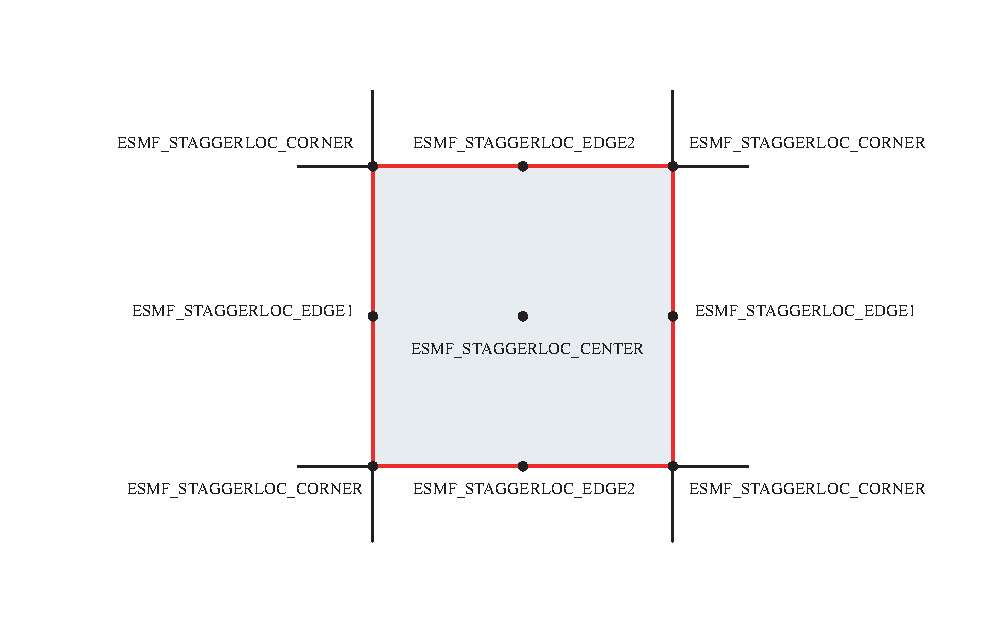
\includegraphics{GridStaggerLoc2D}}
\caption{2D Predefined Stagger Locations}
\label{fig:gridstaggerloc2d}
\end{figure}
\end{center}

The 2D predefined stagger locations (illustrated in figure~\ref{fig:gridstaggerloc2d}) are:\\
\begin{description}
\item [ESMF\_STAGGERLOC\_CENTER:] The center of the cell.
\item [ESMF\_STAGGERLOC\_CORNER:] The corners of the cell.
\item [ESMF\_STAGGERLOC\_EDGE1:] The edges offset from the center in the 1st dimension.
\item [ESMF\_STAGGERLOC\_EDGE2:] The edges offset from the center in the 2nd dimension.
\end{description}

\medskip

\begin{center}
\begin{figure}
\center
\scalebox{1.0}{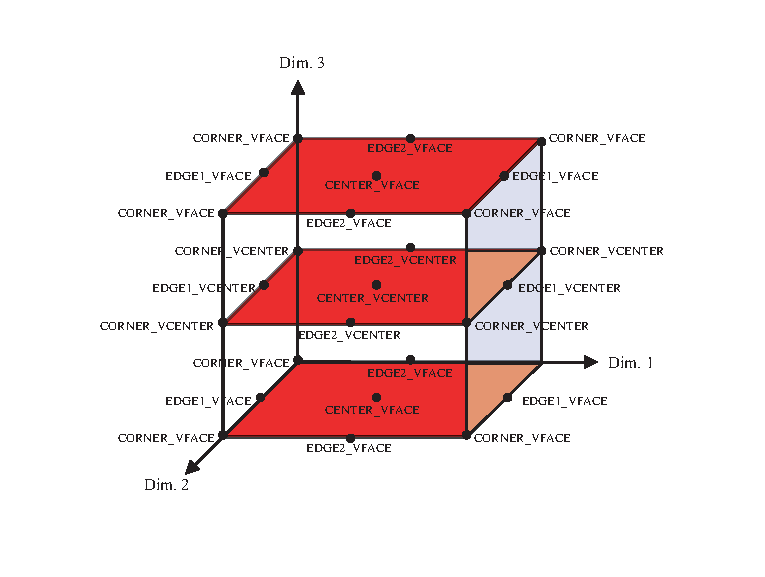
\includegraphics{GridStaggerLoc3D}}
\caption{3D Predefined Stagger Locations}
\label{fig:gridstaggerloc3d}
\end{figure}
\end{center}

The 3D predefined stagger locations (illustrated in figure~\ref{fig:gridstaggerloc3d}) are:\\
\begin{description}
\item [ESMF\_STAGGERLOC\_CENTER\_VCENTER:] The center of the 3D cell.
\item [ESMF\_STAGGERLOC\_CORNER\_VCENTER:] Half way up the vertical edges of the cell.
\item [ESMF\_STAGGERLOC\_EDGE1\_VCENTER:] The center of the face bounded by edge 1 and the vertical dimension.
\item [ESMF\_STAGGERLOC\_EDGE2\_VCENTER:] The center of the face bounded by edge 2 and the vertical dimension. 
\item [ESMF\_STAGGERLOC\_CORNER\_VFACE:] The corners of the 3D cell.
\item [ESMF\_STAGGERLOC\_EDGE1\_VFACE:] The center of the edges of the 3D cell parallel offset from the center in the 1st dimension.
\item [ESMF\_STAGGERLOC\_EDGE2\_VFACE:] The center of the edges of the 3D cell parallel offset from the center in the 2nd dimension.
\item [ESMF\_STAGGERLOC\_CENTER\_VFACE:] The center of the top and bottom face. The face bounded by the 1st and 2nd dimensions. 
\end{description}

\subsubsection{ESMF\_FILEFORMAT}
\label{const:grid:fileformat}

{\sf DESCRIPTION:\\}
This option is used by {\tt ESMF\_GridCreate} to specify the type of the input grid file.  See 
sections~\ref{sec:fileformat:scrip} and \ref{sec:fileformat:gridspec} for more detailed description of the supported file formats.

The type of this flag is:

{\tt type(ESMF\_FileFormat\_Flag)}

The valid values are:
\begin{description}
\item [ESMF\_FILEFORMAT\_SCRIP] SCRIP format grid file. The SCRIP format is the format accepted by the SCRIP regridding tool~\cite{ref:SCRIP}.   For Grid creation, files of this type only work when the {\tt grid\_rank} in the file is equal to 2.

\item [ESMF\_FILEFORMAT\_GRIDSPEC] a single tile grid file comforming with the proposed CF-GRIDSPEC conventions.
\end{description}

